\documentclass[arial,english,brazil,oneside]{estilo/estilo_ifes}

\usepackage[alf]{abntex2cite}
\usepackage[utf8]{inputenc}
\usepackage{lastpage}           % Usado pelo exemplo de ficha catalográfica
\usepackage{microtype}          % para melhorias de justificação
\usepackage{morefloats}         % permite mais floats
\usepackage{listings}
\usepackage{blindtext}          % para gerar texto aleatório (dummy text)
\usepackage{tikz}
\usetikzlibrary[topaths]
\usepackage{mathtools}
\usepackage{float}
\usepackage{setspace}
\usepackage{quoting}
\usepackage{setspace}% http://ctan.org/pkg/{setspace,lipsum}
\usepackage{color, graphicx}
\usepackage[T1]{fontenc}
\usepackage[brazil]{babel}
\usepackage{caption} % Pacote para formatar legendas das figuras e tabelas
\usepackage{url}
\usepackage{enumitem}
\usepackage[justification=centering]{caption}

%\setlist{parsep=\parskip,leftmargin=1.5cm}
\renewcommand{\baselinestretch}{1.5}
%%% Definição da linguagem padrão do documento (pacote babel) para
%%% definir que certas porções do texto (como o resumo, por exemplo)
%%% estão em uma língua estrangeira, usar as macros
%%% \foreignlanguage{languageB}{Text in another language}
%%% ou
%%% \begin{otherlanguage}{languageB}
%%% ...
%%% \end{otherlanguage}
\selectlanguage{brazil}


%%% Define que todos os códigos fontes construídos com o ambiente
%%% `lstlisting' terão uma borda simples.
\lstset{frame=single}


\newcommand{\ifestex}{\textsf{Ifes$7$}}

\titulo{DESENVOLVIMENTO DE APLICATIVO PARA PROMOVER INTEGRAÇÃO\\ENTRE PAIS E ALUNOS NO CONTEXTO EDUCACIONAL}

\autor{FERNANDO RIBEIRO GARIOLI}
\autorficha{GARIOLI, FERNANDO}

\orientador{DSc. Rafael Vargas Mesquita dos Santos}


\instituicao{INSTITUTO FEDERAL ESPÍRITO SANTO}

\curso{Sistemas de Informação}

\data{2019}

\local{Cachoeiro de Itapemirim}

\preambulo{Trabalho de Conclusão de Curso apresentado à Coordenadoria
  do Curso de Sistemas de Informação do Instituto Federal do Espírito
  Santo, Campus Cachoeiro de Itapemirim, como requisito parcial para a obtenção do
  título de Bacharel em Sistemas de Informação.}

\tipotrabalho{Trabalho de Conclusão de Curso}


\begin{document}



\imprimircapa

\imprimirfolhaderosto*

%\begin{fichacatalografica}
  \vspace*{\fill}
  % Posição vertical
  \begin{center}
    % Minipage Centralizado
    \fbox{
      \begin{minipage}[t]{12.5cm}
        \vspace*{3mm}
        \begin{minipage}[t]{2cm}
          X000x
        \end{minipage}
        \begin{minipage}[t]{10cm}
          \imprimirautorficha.\vspace{2mm}

          \hspace{0.5cm}\imprimirtitulo\ / \imprimirautor. ---
          \imprimirlocal, \imprimirdata.\\ 

          \hspace{0.5cm}\pageref{LastPage} p.:\ il. (algumas color.);
          30 cm.\\ 

          \hspace{0.5cm}\imprimirorientadorRotulo~\imprimirorientador.\\

          \hspace{0.5cm}\imprimirtipotrabalho\ ---
          \imprimirinstituicao, \imprimirdata\\

          \hspace{0.5cm}        
          1. Palavra-chave1.
          2. Palavra-chave2.
          I. Orientador.
          II. Universidade xxx.
          III. Faculdade de xxx.
          IV. Título.
          
          \begin{flushright}
            CDU 00:000:000.0
          \end{flushright}
          \vspace*{1mm}
        \end{minipage}
      \end{minipage}
    }
  \end{center}
\end{fichacatalografica}
%
%%% ====================================================================
%%% Exemplo de construção da folha de aprovação. Depois da
%%% apresentação do trabalho, quando a folha de apresentação real
%%% tiver sido assinada pela banca, a folha real deve ser digitalizada
%%% e o ambiente abaixo deve ser substituído por:
%%% \includepdf{folhadeaprovacao_final.pdf}
\begin{folhadeaprovacao}
  \begin{center}
    {\ABNTEXchapterfont\MakeTextUppercase{\imprimirautor}}\\
    \begin{center}
      \ABNTEXchapterfont\MakeTextUppercase{\imprimirtitulo}\\
    \end{center}
    \hspace{.45\textwidth}
    \begin{minipage}{.5\textwidth}
      {\footnotesize{\imprimirpreambulo}}\\
    \end{minipage}%
  \end{center}
  \vspace{-1cm}%
  \begin{center}
    Aprovado em 26 de Novembro de 2019.\\[15mm]
    \textbf{COMISSÃO EXAMINADORA}\\[5mm]
    \assinatura{\imprimirorientador \\
      Instituto Federal do Espírito Santo - Cachoeiro de Itapemirim \\ Orientador}\vspace{-1cm}
    \assinatura{DSc. Eros Estevão de Moura \\
      Instituto Federal do Espírito Santo - Cachoeiro de Itapemirim}\vspace{-1cm}
    \assinatura{MSc. Flávio Izo\\
      Instituto Federal do Espírito Santo - Cachoeiro de Itapemirim}\vspace{-1cm}
  \end{center}
\end{folhadeaprovacao}
%%%% --------------------------------------------------------------------
%%% Ambiente para escrita da declaração do autor
\begin{declaracaodoautor}

  \vspace*{1.5cm}

  Declaro, para fins de pesquisa acadêmica, didática e
  técnico-científica, que este Trabalho de Conclusão de Curso pode ser
  parcialmente utilizado, desde que se faça referência à fonte e ao
  autor.

  \vspace*{2.5cm}

  \centering

  \imprimirlocal, 21 de Novembro de 2019.

  \vspace*{2.5cm}

  \imprimirautor

  \vspace*{\fill}
  
\end{declaracaodoautor}

%%%% ====================================================================
%%% Ambiente para a escrita da dedicatória.
\begin{dedicatoria}
  \vspace*{\fill}
  \hspace{0.2\textwidth}
  \begin{minipage}{0.8\textwidth}
 Dedico esse trabalho primeiramente a Deus, que até aqui tem me sustentado, e a meu avô, Jefferson Ribeiro Viana.
  \end{minipage}
\end{dedicatoria}
%%%% ====================================================================
%%% Agradecimentos
\begin{agradecimentos}
Agradeço primeiramente a Deus, que até aqui tem me sustentado, me dando força e sabedoria para superar as adversidades.

Em segundo, agradeço a minha família, em especial aos meus pais, Henrique e Rosemere, que sempre me ajudaram quando preciso, e sem os quais este momento também não seria possível.

Aos amigos Gideão e Yuri, que me acompanharam durante toda essa jornada.

Aos professores do Ifes, que sempre desejaram para nós o melhor, minha gratidão por toda a dedicação e conselhos oferecidos. Menção honrosa aos professores Bruno Missi, Eros Moura, Flávio Izo, Everson Borges e João Paulo de Brito, grandes espelhos para mim.

Ao meu orientador e amigo, professor Rafael Vargas, a quem conheço desde os tempos de curso técnico, que sempre me incentivou e inspirou a fazer sempre o melhor.

\end{agradecimentos}
%%%% ====================================================================
%%% Epígrafe
\begin{epigrafe}
  \vspace*{\fill}
  \begin{otherlanguage}{english}
    \begin{flushright}
      \begin{SingleSpace}
      "Clama a mim, e responder-te-ei, e anunciar-te-ei coisas grandes e firmes que não sabes".\\ 
      Jeremias 33:3
      \end{SingleSpace}
    \end{flushright}
  \end{otherlanguage}
\end{epigrafe}
%%% Ambiente para resumo em português
\begin{resumo}
    Este trabalho apresenta uma proposta para o desenvolvimento de um aplicativo \textit{mobile} que visa possibilitar o acesso, em tempo real, a dados acadêmicos de alunos de uma rede municipal de ensino, visando a facilitação da participação e engajamento dos responsáveis na vida acadêmica dos alunos. A aplicação possibilita também, através de um módulo baseado em redes neurais, a classificação de um aluno conforme as áreas de conhecimento definidas na reforma do ensino médio brasileiro. A rede utilizada no módulo desenvolvido obteve uma taxa de 94\% de acerto na classificação dos alunos. O aplicativo proposto foi avaliado por alunos do ensino médio através de formulário de pesquisa, obtendo uma média de aprovação de 88\%.
    
    Palavras-chave: educação, tics, redes neurais.
\end{resumo}
%%% Ambiente para resumo em inglês.
\begin{resumo}[Abstract]
    \begin{otherlanguage}{english}
        This work presents a mobile application development proposal, that aims to provide real-time access to a municipal teaching network academic students data, aimingat facilitating the participation and engagement of those responsible in the studentsacademic life. The application also enables, through a module based on neural networks,the classification of a student according to the areas of knowledge defined in the reformof Brazilian high school. The network used in the developed code obtained a rate of 94\% in the students classification.  The proposed application was evaluated by highschool students through the research form, obtaining an average of 88\% approval.
        
        Keywords: education, tics, neural networks.
    \end{otherlanguage}
\end{resumo}

% 

%%% Lista de figuras
\renewcommand{\listfigurename}{Lista de figuras}
\pdfbookmark[0]{\listfigurename}{lof}
\lstlistoflistings*
\cleardoublepage
%%% Lista de figuras
\renewcommand{\listfigurename}{Lista de figuras}
\pdfbookmark[0]{\listfigurename}{lof}
\listoffigures*
\cleardoublepage
%%% Lista de tabelas
\pdfbookmark[0]{\listtablename}{lot}
\listoftables*
\cleardoublepage
%%% Lista de quadros
\pdfbookmark[0]{\listadequadrosname}{loq}
\listadequadros*
\cleardoublepage
%%%% Lista de abreviaturas
\begin{abreviaturas}
\item Item 1
\item Item 2
\item Item 3
\item Item 4
\item Item 5

\end{abreviaturas}

%%%% Lista de símbolos
\begin{simbolos}
\simb{$\Gamma$} Letra grega Gama
\simb{$\Lambda$} Lambda
\simb{$\zeta$} Letra grega minúscula zeta
\simb{$\in$} Pertence
\simb{$\top$} Valor lógico máximo dentro de um reticulado regular
  booleano ou quasi-booleano.
\end{simbolos}
\cleardoublepage


%%% Sumário --- Table of Contents
\pdfbookmark[0]{\contentsname}{toc}
\tableofcontents*
\cleardoublepage

\mainmatter

\include{1-Introcucao}
% ----------------------------------------------------------------------

\chapter{\textbf{Fundamentação Teórica}} % Este comando é utilizado para criar capítulos
\sloppy % Corrige estouro de linhas

\section{TECNOLOGIA NA EDUCAÇÃO}

O termo ``tecnologia'' diz respeito a muitas outras coisas além das máquinas. O conceito tecnologia engloba a criatividade engenhosa do cérebro humano desde os primórdios da Humanidade. Sua aplicação perpassa pela utilização de diversos recursos naturais, com objetivo de criar ferramentas instrumentais e simbólicas, para transpor barreiras impostas pela natureza até aos testes e aplicação de novas teorias e princípios científicos \cite{kenski2007educaccao}.

A sociedade contemporânea está inserida no momento de constante advento tecnocientífico, e de forma direta e indireta, isto reflete nas práticas pedagógicas escolares. Conforme \citeonline{martins2010gestao}, o educador deve estar sempre atualizado, pois a transformação nos processos tecnológicos e meios de comunicação são permanentes. A presença das TIC (tecnologias de informação e comunicação) na educação é um tema dinâmico e catalisador de transformações no processo ensino-aprendizagem. Estudos demonstram que a condição para o uso com êxito das TIC nas escolas reside, antes de tudo, em saber com utilizá-las e aplicá-las nas atividades curriculares \cite{noeth2004evaluating}. Nesse sentido, a qualificação profissional para o uso das TIC é primordial \cite{david2008padroes}.

De acordo com \citeonline{kenski2007educaccao}, a abordagem didática com integração das TIC no processo ensino-aprendizagem pode alavancar a aprendizagem e o desenvolvimento dos educandos via inserção digital. O grande desafio para escola e educadores, consiste em saber aplicar as TIC como potencializador no sistema educacional, especialmente em seus componentes pedagógicos e processos de ensino-aprendizagem \cite{libaneoorganizacao}.

\citeonline[p. 55]{moran2000novas}, apresenta uma perspectiva promissora quanto aos benefícios do emprego da tecnologia no contexto educacional, destacando sua contribuição para a otimização e modernização de metodologias e processos estruturais e sociais deste meio:

\begin{citacao}
    Caminhamos para formas de gestão menos centralizadas, mais flexíveis, integradas. Para estruturas mais enxutas. Menos pessoas, trabalhando mais sinergicamente. Haverá maior participação dos professores, alunos, pais, da comunidade na organização, no gerenciamento, nas atividades, nos rumos de cada instituição escolar.
\end{citacao}

Ao passo dos avanços que se obtêm com o emprego da tecnologia na educação, destacam-se também as Novas Tecnologias de Informação e Comunicação (NTICs), que assumem um papel substancial, fornecendo uma infraestrutura de comunicação que contribui cada vez mais para o aperfeiçoamento da interação dos indivíduos que as utilizam \cite{velloso2014informatica}. Neste advento, dentre varias ferramentas, evidencia-se a internet como um grande instrumento catalisador, sendo capaz de contribuir inclusive na motivação dos alunos no processo de aprendizagem \cite{moran1997utilizar}.

\subsection{Trabalhos relacionados}

No âmbito da educação, várias ferramentas têm sido utilizadas como instrumento de auxílio na aprendizagem, bem como na aproximação do aluno com a escola. Tais instrumentos promovem novas possibilidades de interação didático pedagógicas, permitindo a troca e a disponibilização de informações de forma ágil e funcional entre alunos e docentes \cite{medeiros2018educaccao}.

A tabela \ref{tabela:comparacao} demonstra um comparativo de características básicas entre o aplicativo proposto neste trabalho e outras 4 aplicações similares: 

\begin{table}[H]
    \small
	\centering
	\caption{Comparativo de características com ferramentas similares.}
	\renewcommand{\arraystretch}{1.8}
	\begin{tabular}{>{\centering}m{1.7in} >{\centering}m{0.7in} >{\centering}m{0.7in} >{\centering}m{0.7in} >{\centering}m{0.7in} >{\centering\arraybackslash}m{0.7in}}
	    \hline
		\multicolumn{1}{c|}{\textbf{\parbox{1.7in}{\centering Característica}}}
		& \multicolumn{1}{c|}{\textbf{\parbox{0.7in}{\centering Aplicativo proposto}}}
		& \multicolumn{1}{c|}{\textbf{\parbox{0.7in}{\centering ClassApp}}}
		& \multicolumn{1}{c|}{\textbf{\parbox{0.7in}{\centering Escola Direta}}}
		& \multicolumn{1}{c|}{\textbf{\parbox{0.7in}{\centering Escola Web}}}
		& \multicolumn{1}{c}{\textbf{\parbox{0.7in}{\centering Connect Escolas}}} \\
	    \hline
	\end{tabular}
	\renewcommand{\arraystretch}{1.5}
	\begin{tabular}{>{\centering}m{1.7in} >{\centering}m{0.7in} >{\centering}m{0.7in} >{\centering}m{0.7in} >{\centering}m{0.7in} >{\centering\arraybackslash}m{0.7in}}
	    Acesso a frequência, notas e boletim & X & X & X & X & X \\
		Calendário/Eventos & X & X & X & X & X \\
		Mensagens/Comunicados & X & X & X & X & X \\
        Cardápio Nutricional & &  & X & & \\
        Gratuito & X & & & &  \\
        Open Source & X & & & & \\
		\hline
	\end{tabular}
	\label{tabela:comparacao}
	\captionsetup{singlelinecheck = false, format= hang, justification=raggedright, labelsep=space, width=6.25in}
	\caption*{\footnotesize Fonte: O Autor.}
\end{table}

\section{NOVO ENSINO MÉDIO}

O movimento de reformulação do currículo do ensino médio não é recente. Já no período imediatamente após ter sido sancionada a LDB (Lei de Diretrizes e Bases), em conformidade o que determina o artigo 26, o Conselho Nacional de Educação (CNE) dando início à produção das Diretrizes Curriculares Nacionais para as etapas e modalidades da educação básica. Desde então, são várias as iniciativas de reformulação curricular do ensino médio \cite{lei9394}. Do que afirma a LDB para o currículo do ensino médio, destaca-se o art. 36:

\begin{citacao}
    O currículo do ensino médio observará o disposto na Seção I deste capítulo e as seguintes diretrizes:

    I – destacará a educação tecnológica básica, a compreensão do significado da ciência, das letras e das artes; o processo histórico de transformação da sociedade e da cultura; a língua portuguesa como instrumento de comunicação, acesso ao conhecimento e exercício da cidadania;
    
    II – adotará metodologias de ensino e de avaliação que estimulem a iniciativa dos estudantes;
    
    I – domínio dos princípios científicos e tecnológicos que presidem a produção moderna;
    
    § 2º - O ensino médio, atendida a formação geral do educando, poderá prepará-lo para o exercício de profissões técnicas.
    
    § 4º - A preparação geral para o trabalho e, facultativamente, a habilitação profissional, poderão ser desenvolvidas nos próprios estabelecimentos de ensino médio ou em cooperação com instituições especializadas em educação profissional. \cite{lei9394}.
\end{citacao}

Conforme a Lei 13.415/17 \cite{lei13415}, a Base Nacional Comum Curricular (BNCC) define direitos e objetivos de aprendizagem do ensino médio, conforme diretrizes do Conselho Nacional de Educação, nas áreas de linguagens e suas tecnologias; matemática e suas tecnologias; ciências da natureza e suas tecnologias e ciências humanas e sociais aplicadas, tal como mostra a figura \ref{figura:novo_ensino_medio}:

\begin{figure}[H]
	\caption{Novo Ensino Médio separado por áreas de conhecimento.}
	\centering % para centralizarmos a figura
	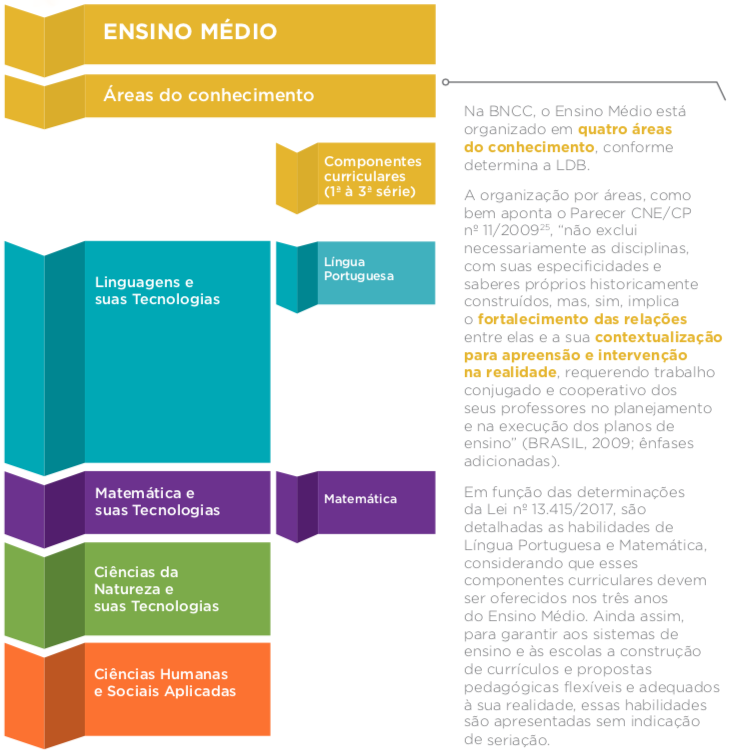
\includegraphics[width=14cm]{resources/novo_ensino_medio.png} % leia abaixo
	\label{figura:novo_ensino_medio}
	\captionsetup{singlelinecheck = false, format= hang, justification=raggedright, labelsep=space, width=14cm}
	\caption*{\footnotesize Fonte: \citeonline{bncc2018}.}
\end{figure}

Mediante a toda essa concepção e mesmo revolução, o Novo Ensino Médio foi pensado para atender as diversas juventudes que se apresentam na escola. As mudanças propostas são definidas a partir da Lei nº 13.415, de 2017, e delineadas nas Diretrizes Curriculares para o Ensino Médio \cite{res32016}.

\section{REDES NEURAIS ARTIFICIAIS}

\subsection{CONCEITO}

\citeonline{haykin2009neural} descreve o conceito de Redes Neurais Artificiais (RNA) utilizando-se do exemplo dos sistemas biológicos naturais, que possuem alta capacidade de aprendizado e conseguem assimilar informações complexas no ambiente ao redor em um curto espaço de tempo. Isto se dá pelo fato de que um computador processa informações de forma diferente de um cérebro humano, por exemplo. Neste escopo, uma rede neural objetiva o mapeamento de tais informações de forma a torná-las acessíveis para utilização, tal como afirma \citeonline[p. 28]{haykin2007redes}:

\begin{citacao}
	Uma rede neural é um processador maciçamente paralelamente distribuído constituído de unidades de processamento simples, que têm a propensão natural para armazenar conhecimento experimental e torná-lo disponível para o uso. Ela se assemelha ao cérebro em dois aspectos:
	\begin{enumerate}[leftmargin=4.7cm, topsep=0cm]
	    \item O conhecimento é adquirido pela rede a partir de seu ambiente através de um processo de aprendizagem.
	    \item Forças de conexão entre neurônios, conhecidas como pesos sinápticos, são utilizadas para armazenar o conhecimento adquirido.
	\end{enumerate}
\end{citacao}

Para \citeonline{hagan1996neural}, apesar de as as Redes Neurais não apresentarem uma solução para todos os problemas matemáticos e de engenharia, elas tem se mostrado um recurso poderoso em casos apropriados para sua aplicação. Muitos dos seus avanços atuais se devem ao avanço do poder de processamento dos computadores, o que possibilita a realização de testes cada vez mais complexos.

\subsection{MODELO DE ORGANIZAÇÃO}

Considerando o modelo de organização de uma Rede Neural Artificial (RNA), existem duas características básicas que a definem, sendo estas sua arquitetura e seu modelo de aprendizagem. Para que uma RNA funcione, se faz necessário um treinamento prévio através de dados de exemplo fornecidos, que serão levados como parâmetro para uma classificação de resultados. Neste sentido, através dos parâmetros obtidos, são atribuídos pesos para cada tipo de informação de entrada a ser processada pela rede \cite{thomas2019}.

O neurônio artificial, definido por \citeonline{mcculloch1943logical}, representa uma unidade de processamento de uma RNA, sendo de considerada de importância fundamental para o funcionamento da rede \cite{haykin2007redes}. A primeira aplicação prática de um neurônio artificial foi concebida por \citeonline{rosenblatt1958perceptron} com a rede \textit{perceptron}, capaz de realizar reconhecimento de padrões.

A figura \ref{figura:modelo_neuronio} representa o modelo de um neurônio artificial, constituído de entradas predefinidas (x\textsubscript{1}, x\textsubscript{2}, x\textsubscript{D}), que têm o seu valor multiplicado por um peso (w\textsubscript{1}, w\textsubscript{2}, w\textsubscript{D}), indicando o grau de importância da respectiva entrada. Tais valores são somados através de uma combinação linear e encaminhados em seguida para uma função de ativação. A partir de então, é verificado se o valor produzido pela função atinge um limiar \(\mu\). Caso o resultado ultrapasse o limiar definido, o neurônio produz uma saída positiva \cite{thomas2019}.

\begin{figure}[H]
	\caption{Modelo de neurônio artificial de McCulloch e Pitts.}
	\centering % para centralizarmos a figura
	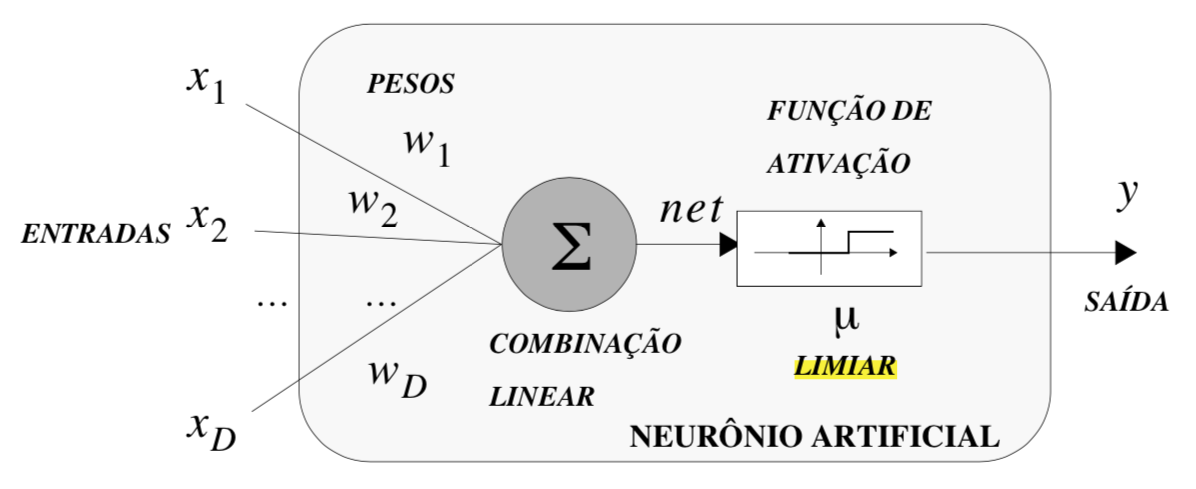
\includegraphics[width=12cm]{resources/modelo_neuronio.png} % leia abaixo
	\label{figura:modelo_neuronio}
	\captionsetup{singlelinecheck = false, format= hang, justification=raggedright, labelsep=space, width=12cm}
	\caption*{\footnotesize Fonte: \citeonline{thomas2019}.}
\end{figure}

\subsection{SINGLE LAYER PERCEPTRON X MULTILAYER PERCEPTRON}

Quanto a organização de uma Rede Neural Artificial, \citeonline{fausett1994fundamentals} descreve os arranjos de RNA's em camadas. Uma RNA com apenas uma camada é denominada uma \textit{Single Layer Perceptron}, ao passo que uma RNA com múltiplas camadas é denominada uma \textit{Multilayer Perceptron}.

O uso de RNA's do tipo \textit{Single Layer Perceptron} se remete a problemas de ordem linear \cite{haykin2009neural}, como apresenta a figura \ref{figura:perceptron_binary}, onde duas classes de informações (+ e -), podem ser separadas por uma única reta. Tais problemas permitem a classificação de dados de entrada em até duas categorias, limitando sua aplicação à problemas mais complexos, o que pode exigir aplicação de uma rede multicamada (\textit{Multilayer Perceptron}) \cite{fausett1994fundamentals}.

\begin{figure}[H]
	\caption{Exemplo de separação linear binária.}
	\centering % para centralizarmos a figura
	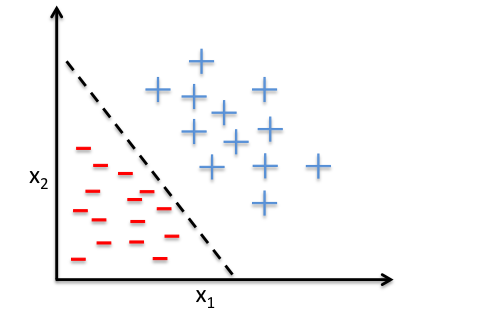
\includegraphics[width=11cm]{resources/perceptron_binary.png} % leia abaixo
	\label{figura:perceptron_binary}
	\captionsetup{singlelinecheck = false, format= hang, justification=raggedright, labelsep=space, width=11cm}
	\caption*{\footnotesize Fonte: \citeonline{2015_singlelayer}.}
\end{figure}

Em uma rede \textit{Multilayer Perceptron}, tal como representado na figura \ref{figura:multilayer_perceptron}, o emprego de várias camadas é utilizado para possibilitar a separação de elementos que uma rede \textit{Single Layer Perceptron} não é capaz de realizar. Neste modelo, os perceptrons utilizam-se de funções de ativação não-lineares, que tornam possível tal refinamento no processo \cite{marius2009}.

\begin{figure}[H]
	\caption{Exemplo de separação linear não-binária.}
	\centering % para centralizarmos a figura
	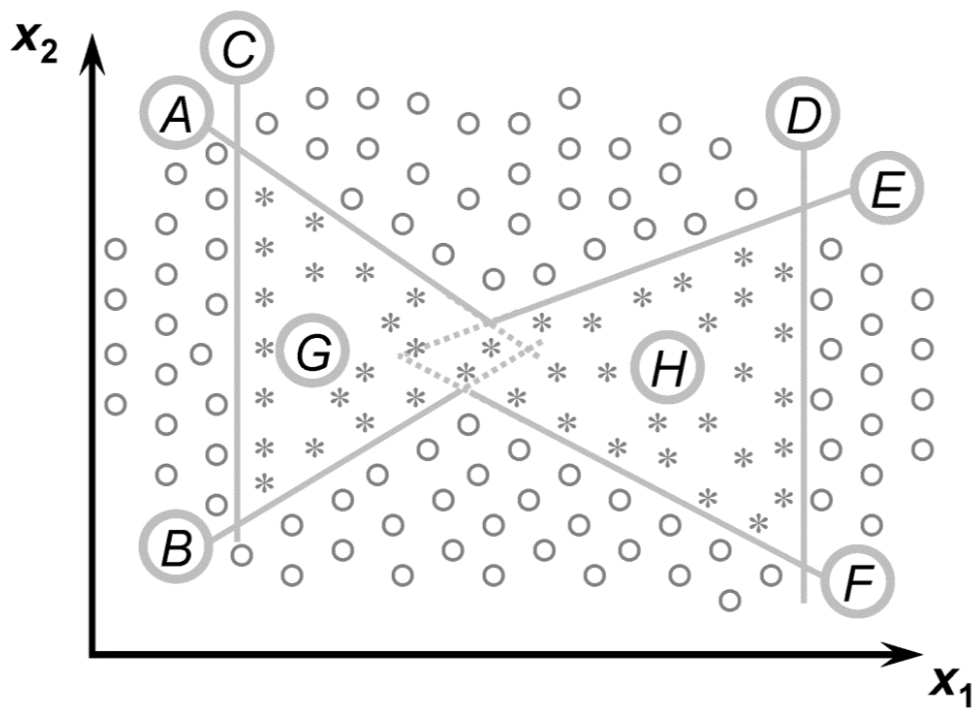
\includegraphics[width=9.5cm]{resources/multilayer_perceptron.png} % leia abaixo
	\label{figura:multilayer_perceptron}
	\captionsetup{singlelinecheck = false, format= hang, justification=raggedright, labelsep=space, width=9.5cm}
	\caption*{\footnotesize Fonte: \citeonline{da2010redes}.}
\end{figure}

\subsection{APRENDIZAGEM SUPERVISIONADA}

Quanto ao processo de aprendizagem de uma RNA, os métodos de aprendizagem podem ser classificados como supervisionados e não-supervisionados \cite{haykin2007redes}. Na ocasião do procedimento supervisionado, há um ambiente de treinamento contendo modelos de saída já conhecidos e classificados, utilizados como parâmetro para classificação \cite{marius2009}.

\citeonline{2014_supervised_learning} exemplifica a aprendizagem supervisionada descrevendo um sistema de filtragem de \textit{spam}, no qual ao visualizar um \textit{e-mail} uma pessoa saberia identificá-lo como uma mensagem de lixo eletrônico. A partir de então, seria possível reunir informações características de mensagens do mesmo tipo para classificar outras mensagens ainda não visualizadas.

Em RNA's com modelo de aprendizagem não-supervisionado, ao contrário do modelo supervisionado, não são utilizados modelos explícitos de saída para o treinamento, e nenhuma avaliação da mesma é realizada \cite{von2005rede}. Neste caso, a própria rede deve identificar os modelos de aprendizagem e criar novos, caso necessário \cite{becker1991}.

\subsection{WEKA}

\textit{Weka} \cite{hall2009weka}, é uma ferramenta com foco em \textit{machine learning} que reúne uma gama de algoritmos de \textit{data mining}. Juntamente com os algoritmos, a ferramenta provê utilitários para preparação, classificação, regressão, clusterização, associação e visualização de dados, de modo a tornar o processo de mineração de dados mais aprimorado.

Com Weka, é possível aplicar um algoritmo de aprendizagem para um conjunto de dados e analisar os resultados do processo, de modo a facilitar a identificação de possíveis padrões sobre o dados analisados \cite{eibe2016weka}. Construído em linguagem Java, também possibilita sua inclusão como biblioteca em \textit{softwares} que porventura venham a utilizar tais recursos da ferramenta. A figura \ref{figura:weka_explorer} demonstra a interface gráfica do \textit{Weka Explorer}:

\begin{figure}[H]
	\caption{Interface do \textit{Weka Explorer}.}
	\centering % para centralizarmos a figura
	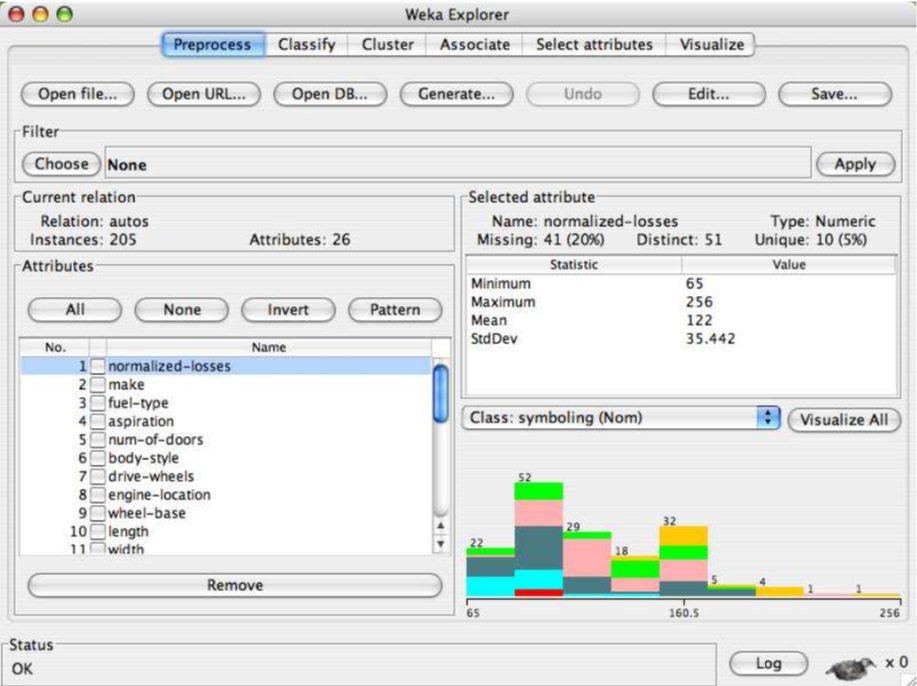
\includegraphics[width=13cm]{resources/weka.png} % leia abaixo
	\label{figura:weka_explorer}
	\captionsetup{singlelinecheck = false, format= hang, justification=raggedright, labelsep=space, width=13cm}
	\caption*{\footnotesize Fonte: \citeonline{hall2009weka}.}
\end{figure}

\section{TECNOLOGIAS EMPREGADAS}

\subsection{SISTEMAS DISTRIBUÍDOS}

Na computação moderna vários sistemas computacionais interagem entre si de forma interdependente, sendo a internet o exemplo mais perceptível a ser citado. São várias redes interconectadas e aplicações que fazem uso de tais estruturas para se comunicarem, abrangendo os mais variados domínios. Todas essas estruturas empregam conceitos da tecnologia sistemas distribuídos \cite{puder2011distributed}.\\
\citeonline{tanenbaum2007distributed} descrevem um sistema distribuído como sendo um conjunto de computadores autônomos não obrigatoriamente equivalentes, interligados entre si e compreendidos pelo usuário como um único sistema conexo. Sua compreensão destaca a interdependência e a colaboração entre os computadores como sendo um elemento de suma importância para a existência da arquitetura. A definição proposta por \citeonline[p. 2]{coulouris2005distributed} torna ainda mais precisa através da seguinte definição sobre sistemas distribuídos:

\begin{citacao}
	Definimos um sistema distribuído como aquele no qual os componentes de hardware ou software, localizados em computadores interligados em rede, comunicam-se e coordenam suas ações apenas enviando mensagens entre si.
\end{citacao}

\citeonline{puder2011distributed} destacam vários benefícios dos sistemas distribuídos em comparação com sistemas centralizados, tais como redundância, economia, escalabilidade e tolerância a falhas.

\subsection{WEB SERVICES}

Considerando as várias utilidades dos sistemas distribuídos, \citeonline{fielding2000} definiu em sua tese de doutorado o \textit{REpresentational State Transfer} (REST), um estilo arquitetônico para sistemas hipermídia distribuídos. Tal arquitetura foi desenvolvida com base na disponibilização de recursos, mapeados de forma exclusiva através de URIs (\textit{Uniform Resource Identifiers}), que são acessadas através de URLs (\textit{Uniform Resource Location}), funcionando sobre o protocolo HTTP \cite{richardson2008restful}. Em seu trabalho, Fielding destaca seis atribuições básicas que caracterizam o padrão REST, são estas:

\begin{enumerate}
	\item {A aplicação deve utilizar a arquitetura cliente-servidor;}
	\item {Todas as requisições devem ser independentes e isoladas entre si, não havendo nenhum estado de sessão guardado no servidor (\textit{Stateless});}
	\item {Requisições já executadas previamente podem ser mantidas em memória para reutilização futura por chamadas equivalentes (Cache);}
	\item {Deve existir uma padronização na manipulação, no mapeamento dos componentes disponibilizados e no formato de troca de dados (Interface Uniforme);}
	\item {O sistema deve ser projetado em camadas, de modo que a interação entre componentes de diferentes camadas seja limitada ao essencial;}
	\item {Código sob demanda, permitindo que \textit{applets} ou \textit{scripts} sejam baixados para execução no lado cliente (podendo ser opcional a implementação deste quesito);}
\end{enumerate}

O padrão definido por Fielding se mostra uma alternativa altamente performática em comparação com  \textit{web services} tradicionais tais como SOAP, principalmente pelo tamanho de mensagens e tempos de resposta menores, tal como afirmam \citeonline{hamad2010} e \citeonline{dudhe2014performance}. A comunidade web e grandes empresas tais como Google e Amazon têm se utilizado dessa tecnologia para construir seus serviços, dado sua simplicidade e escalabilidade \cite{wagh2014hybrid}. REST tem sido amplamente utilizado em conjunto com o \textit{JavaScript Object Notation} (JSON), uma estrutura de dados simples e leve, em substituição ao formato XML como padrão representativo de troca de dados, sendo suportado pela maioria dos \textit{Web Browsers} atuais \cite{knutsen2018}.

A figura \ref{figura:webservices} ilustra uma representação básica de um \textit{Web Service RESTful} implementado utilizando a arquitetura Rest (RESTful), onde essencialmente são realizadas requisições (HTTP Request) a partir de um determinado cliente (aplicação ou \textit{web browser}) para um servidor (\textit{REST Server}), que responde à solicitação com uma resposta (HTTP Response), contendo em seu corpo uma informação padronizada por algum formato representativo de troca de dados (XML, JSON, HTML, TEXT).

\begin{figure}[H]
	\caption{Arquitetura de um \textit{Web Service RESTful}.}
	\centering % para centralizarmos a figura
	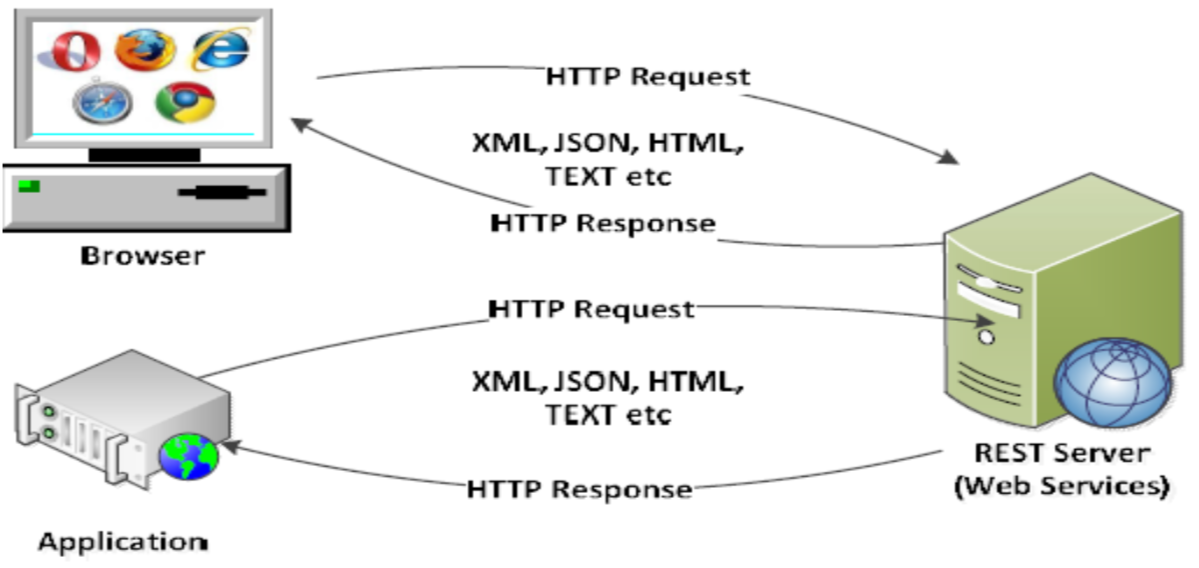
\includegraphics[width=13cm]{resources/webservices.png} % leia abaixo
	\label{figura:webservices}
	\captionsetup{singlelinecheck = false, format= hang, justification=raggedright, labelsep=space, width=13cm}
	\caption*{\footnotesize Fonte: \citeonline{thu2015}.}
\end{figure}

Aplicações \textit{RESTful} utilizam-se dos chamados métodos HTTP para manipulação de dados. A tabela \ref{tabela:metodoshttp} lista os principais métodos e suas respectivas ações, sendo elas leitura, criação, alteração e deleção de dados, respectivamente \cite{pautasso2008restful}.

\begin{table}[H]
    \small
	\centering
	\caption{Métodos HTTP e suas funções correspondentes.}
	\renewcommand{\arraystretch}{1.5}
	\begin{tabular}{>{\centering}m{1.5in} >{\centering\arraybackslash}m{2.0in}}
	    \hline
		\multicolumn{1}{c|}{\textbf{Método HTTP}} 
		& \multicolumn{1}{c}{\textbf{Ação}}\\
		\hline
		GET & Lê um recurso \\
		POST & Cria um recurso \\
		PUT & Altera um recurso \\
        DELETE & Deleta um recurso \\
		\hline
	\end{tabular}
	\label{tabela:metodoshttp}
	\captionsetup{singlelinecheck = false, format= hang, justification=raggedright, labelsep=space, width=9.8cm}
	\caption*{\footnotesize Fonte: \citeonline{hamad2010}.}
\end{table}

\subsection{JSON WEB TOKEN (JWT)}

Quanto à segurança de acesso, \textit{web services RESTful} podem se utilizar de mecanismos para garantir que somente usuários autorizados tenham acesso aos recursos. Neste sentido, o padrão JWT (\textit{JSON Web Token}) \cite{jwt} se mostra uma alternativa concreta para a transmissão de informações confidenciais de autenticação em sistemas \textit{stateless} \cite{jones2015json}. \citeonline{peyrott2016jwt} descreve tal padrão como um meio simples, compacto e seguro de realizar solicitações, sendo utilizado por uma grande parcela de aplicativos. O fato de se utilizar da estrutura JSON se deve a sua ampla adoção pelos  navegadores web modernos \cite{jones2011emerging}.

A figura \ref{figura:jwt} ilustra a estrutura básica do JWT, constituída basicamente por uma string de caracteres criptografada denominada \textit{Token}, dividida em três seções: \textit{header}, \textit{payload} e \textit{signature}.

\begin{figure}[H]
	\caption{Estrutura básica de um \textit{token} JWT.}
	\label{figura:jwt}
	\begin{center}
		\textcolor{red}{xxxxxx}.\textcolor{green}{yyyyyyy}.\textcolor{blue}{zzzzzzzz}\\
		\textcolor{red}{header}.\textcolor{green}{payload}.\textcolor{blue}{signature}\\
	\end{center}
	\caption*{\footnotesize Fonte: \citeonline{rahmatulloh2018}.}
\end{figure}

\citeonline{janoky2018} ressaltam algumas vantagens da utilização de \textit{tokens} JWT, justificando seu uso como forma de controle de acesso a determinadas funções em um sistema distribuído. Destacam-se dentre estas a diminuição da complexidade na utilização do serviço, e o ganho em performance, dado que todas as informações de autenticação e autorização do usuário são inseridas junto ao \textit{token}, o que dispensa a realização de uma chamada ao \textit{web service} para verificar se o usuário logado possui ou não permissão de acesso à uma determinada função.

Na figura \ref{figura:jwt-schema} temos um esquema básico de autenticação e validação de um \textit{token} JWT onde, na fase de autenticação, são encaminhados os dados de login do usuário para o servidor. Caso a validação tenha ocorrido com sucesso, um \textit{token} é gerado e retornado para a aplicação cliente (\textit{Browser} ou Aplicativo), que pode acessar recursos permitidos enquanto o mesmo estiver válido.

\begin{figure}[H]
	\caption{Diagrama de autenticação e validação de \textit{token}.}
	\centering % para centralizarmos a figura
	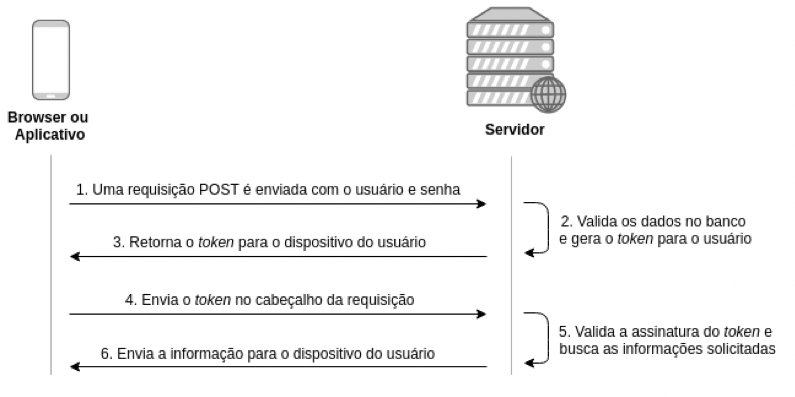
\includegraphics[width=14cm]{resources/jwt-schema.png} % leia abaixo
	\label{figura:jwt-schema}
	\captionsetup{singlelinecheck = false, format= hang, justification=raggedright, labelsep=space, width=14cm}
	\caption*{\footnotesize Fonte: \citeonline{montanheiro2017utilizaccao}.}
\end{figure}


\chapter{\textbf{Metodologia de Pesquisa}} % Este comando é utilizado para criar capítulos
\sloppy % Corrige estouro de linhas

\section{Web Service Restful e Aplicativo}

Para a construção do Web Service Restful e do aplicativo foi utilizado como referência o modelo aplicado na disciplina de Laboratório de Engenharia de Software do curso de Sistemas de Informação do Ifes Campus Cachoeiro, baseado no \textit{Rational Unified Process} (RUP), representado na figura \ref{figura:rup}.

\begin{figure}[h]
	\caption{Processo de desenvolvimento de \textit{software} baseado no RUP.}
	\centering % para centralizarmos a figura
	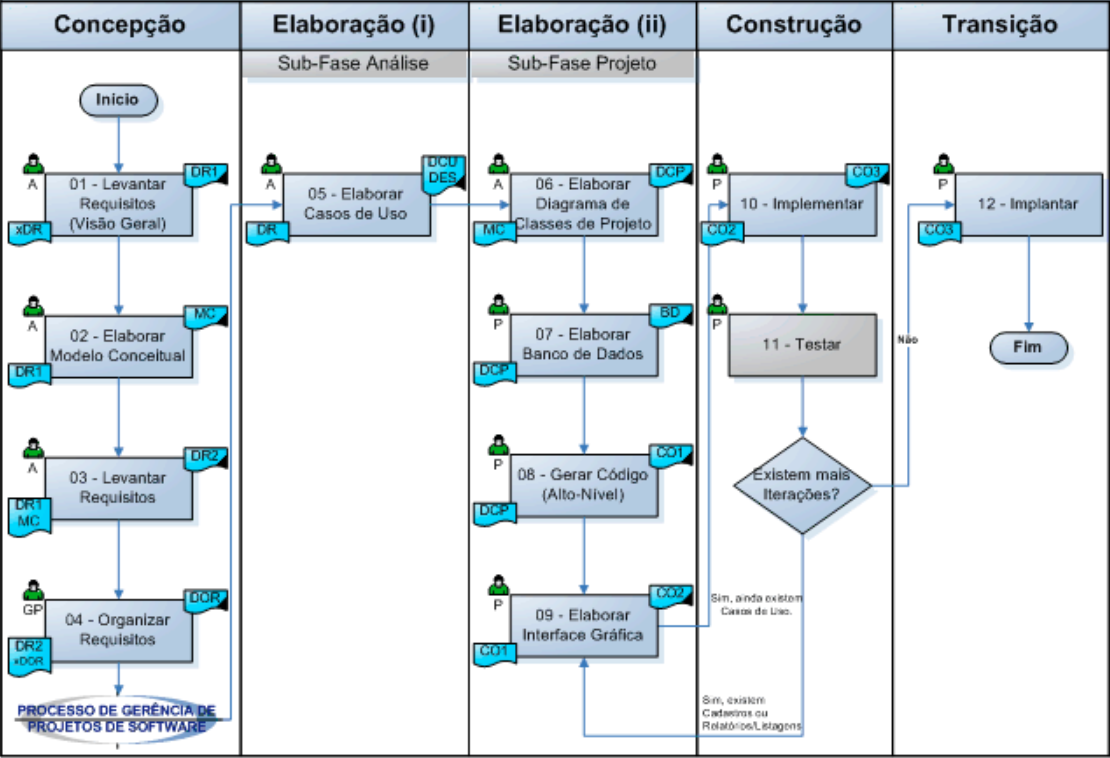
\includegraphics[width=16cm]{resources/pds_rup.png} % leia abaixo
	\label{figura:rup}	
	\caption*{Fonte: \citeonline{rupLes}.}
\end{figure}

Para tal, os seguintes passos descritos no modelo (figura \ref{figura:rup}) foram executados para a elaboração dos \textit{sofwares}:

\begin{enumerate}
   \item Levantar Requisitos (Visão Geral): identificar descrever de forma geral o funcionamento do aplicativo e suas principais funções;
   \item Elaborar modelo conceitual: identificar classes e relacionamentos concernentes ao domínio (nesta fase não se faz necessário a inclusão dos atributos nas classes);
   \item Levantar Requisitos: elaborar documento de requisitos contendo o detalhamento de todas as funcionalidades do aplicativo;
   \item Organizar Requisitos: elaborar documento de organização de requisitos separando todos os requisitos em processos de negócios e relatórios/listagens;
   \item Elaborar banco de dados: 
   \item Elaborar interface gráfica: estruturar todas as telas do aplicativo;
   \item Implementar: codificar as classes necessárias para implementação das funcionalidades de processos de negócio e listagens;
   \item Testar: realizar testes de todas as funcionalidades implementadas;
   \item Implantar: gerar o arquivo instalável do aplicativo (APK) e instalar o \textit{webservice} no servidor de produção;
\end{enumerate}

\section{Módulo de Recomendação}

Para a construção do módulo de recomendação do aplicativo foi utilizado a biblioteca Weka para realizar o treinamento da rede e extrair os resultados do mesmo. Para tanto, a biblioteca utiliza um arquivo do tipo ARFF para descrever os os atributos, as possibilidades de classificação e os respectivos exemplos de classificação utilizados no treinamento em questão. Sua estrutura básica é representada na figura \ref{figura:arff}.

\begin{figure}[h]
	\caption{Sintaxe básica de um arquivo de treinamento utilizado pelo Weka.}
	\centering % para centralizarmos a figura
	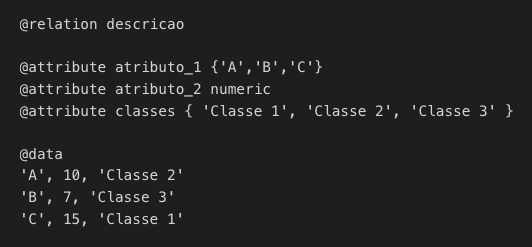
\includegraphics[width=12cm]{resources/arff.png} % leia abaixo
	\label{figura:arff}	
	\caption*{Fonte: O Autor.}
\end{figure}

\break

\section{Ambiente de desenvolvimento}

As seguintes ferramentas e \textit{softwares} foram utilizados no processo de desenvolvimento:

\begin{itemize}
    \item Banco de Dados Oracle (versão 11g);
    \item Java SE \textit{Development Kit} (versão 8 update 221);
    \item Ionic \textit{Framework} (versão 4);
    \item Servidor Web Payara (versão 5.191);
    \item Netbeans IDE (versão 11.1);
    \item Visual Studio Code (versão 1.39.1);
    \item Postman (versão 7.2);
\end{itemize}
\chapter{\textbf{Resultados}} % Este comando é utilizado para criar capítulos
\sloppy % Corrige estouro de linhas

\section{Web Service Restful e Aplicativo}

\subsection{Levantar Requisitos (Visão Geral)}
Nesta etapa foi 

\subsection{Elaborar Modelo Conceitual}

\subsection{Levantar Requisitos}

\subsection{Organizar Requisitos}

\subsection{Elaborar Banco de Dados}

\subsection{Implementar}

\subsubsection{Aplicativo}

\subsubsection{Web Service Restful}

\subsection{Testar}

\subsection{Implantar}

\section{Módulo de Recomendação}
%\chapter{\textbf{Conclusões gerais e trabalhos futuros}} % Este comando é utilizado para criar capítulos

O presente trabalho proporcionou a construção de um aplicativo \textit{mobile} que visa estimular uma maior participação de responsáveis na vida acadêmica de alunos de uma rede municipal de ensino, realizando a integração dos mesmos com a escola. Para tal, o \textit{software} permitiu a visualização em tempo real de dados acadêmicos dos alunos pelos usuários, bem como de mensagens provenientes das escolas e professores. Conjuntamente, foi disponibilizado a possibilidade de classificação de um aluno levando em consideração as áreas de conhecimento do novo ensino médio, visando o auxílio no conhecimento das aptidões acadêmicas do mesmo.

O aplicativo foi avaliado por alunos do ensino médio do Ifes Campus Cachoeiro, obtendo uma média de 88\% de aprovação nos itens considerados através do formulário de pesquisa aplicado. A rede neural elaborada obteve um percentual de 94\% de acerto na classificação de alunos, considerando dados simulados.

Como trabalhos futuros, verificou-se a realização do treinamento da rede neural, considerando dados de classificação real dos alunos, após a implementação do novo ensino médio. Ademais, verificou-se também a possibilidade de implementação, junto à funcionalidade de mensagens, da comunicação por parte dos responsáveis com a escola e com os professores do aluno.

Levando em consideração as tecnologias utilizadas no processo de desenvolvimento, a plataforma construída permite facilmente que possíveis novas funcionalidades sejam incorporadas a ela de maneira ágil.
%%% ====================================================================
%%% Início da parte pós-textual do documento.
\postextual


%%% Referências Bibliográfica

\bibliography{bibliografia/bibliography}

%%%% Início dos apêndices ---------------------------------------------
\apendices


% --------------------------------------------------------------------
\chapter{Titulo}

\begin{enumerate}
    \item Item 1
    \item Item 2
\end{enumerate}

% --------------------------------------------------------------------



%%%% Início dos anexos ------------------------------------------------
\anexos

\partanexos*

\chapter{Exemplo de lombada}

\hspace*{0mm}\fbox{\includegraphics[scale=0.8]{pics/normas-ifes-apendice-d.png}}

\end{document}

